\documentclass[12pt,a4paper]{article}

\usepackage[a4paper,margin=1in]{geometry}
\usepackage[T1]{fontenc}
\usepackage[utf8]{inputenc}
\usepackage{lmodern}
\usepackage{datetime}
\newdateformat{monthyeardate}{\monthname[\THEMONTH]-\THEYEAR}
\usepackage{microtype}
\usepackage{xcolor}
\usepackage{graphicx}
\usepackage{booktabs}
\usepackage{tabularx}
\usepackage{enumitem}
\usepackage{tikz}
\usetikzlibrary{arrows.meta,positioning,shapes.geometric}
\usepackage{listings}
\usepackage{float}
\usepackage{fancyhdr}
\usepackage[hidelinks]{hyperref}

\definecolor{brandpurple}{HTML}{7B0099}
\definecolor{brandgold}{HTML}{F1B400}
\definecolor{codebg}{HTML}{F5F5F6}
\definecolor{codegray}{HTML}{555555}

\hypersetup{
  pdftitle={Ngaithla teh Project Report},
  pdfauthor={Vanlalawmpuia Ralte},
  colorlinks=true,
  linkcolor=brandpurple,
  urlcolor=brandpurple
}

\pagestyle{fancy}
\fancyhf{}
\lhead{Ngaithla teh}
\rhead{Project Report}
\cfoot{\thepage}

\lstset{
  basicstyle=\ttfamily\small,
  backgroundcolor=\color{codebg},
  frame=single,
  rulecolor=\color{black!15},
  breaklines=true,
  columns=fullflexible,
  showstringspaces=false,
  keywordstyle=\color{brandpurple}\bfseries,
  commentstyle=\color{codegray}\itshape,
  stringstyle=\color{black!70}
}

\newcommand{\studentName}{Vanlalawmpuia Ralte (Opa)}
\newcommand{\studentUSN}{U25UV24T029118}
\newcommand{\currentSemester}{V Semester}
\newcommand{\studentBranch}{BTech (CSE)}
\newcommand{\department}{DEPARTMENT OF COMPUTER SCIENCE AND ENGINEERING}
\newcommand{\projectTitle}{NGAITHLA TEH - A MUSIC RATING APP}
\newcommand{\academicYear}{2026-27}
\newcommand{\guideName}{Sangeetha U}
\newcommand{\guideDesignation}{Faculty}
\newcommand{\chairpersonName}{Dr. S H Manjulla}
\newcommand{\chairpersonDesignation}{Professor \& Chairperson}
\newcommand{\projectname}{Ngaithla teh}
\title{\textbf{Ngaithla teh}\\[0.4em]\large Community Music Library}
\author{Vanlalawmpuia Ralte}
\date{September 2026}

\begin{document}

\begin{titlepage}
  \centering
  {\large\bfseries\itshape UNIVERSITY OF VISVESVARAYA COLLEGE OF ENGINEERING\par}
  \vspace{0.1cm}
  {\bfseries\itshape \department\par}
  \vspace{0.1cm}
  {\small\itshape K.R. Circle, Bengaluru -- 560001\par}

  \vspace{4.5cm}
  {\large A DBMS Mini-Project Report on\par}
  \vspace{0.4cm}
  {\Large\bfseries\itshape \projectTitle\par}

  \vspace{3.5cm}
  {\large Submitted by\par}
  \vspace{0.5cm}
  {\large\bfseries\itshape \studentName\ (\studentUSN)\par}
  {\large\bfseries\itshape \currentSemester, \studentBranch\par}

  \vfill
  {\large Under the guidance of\par}
  \vspace{0.5cm}
  {\large\bfseries\itshape \guideName\par}
  {\large\itshape \guideDesignation\par}
  {\large\bfseries\itshape Department of Computer Science and Engineering\par}
  {\large\bfseries\itshape UVCE\par}

  \vfill
  {\large \monthyeardate\today\par}
\end{titlepage}

\clearpage
\pagestyle{empty}

\begin{center}
  {\large\bfseries\itshape UNIVERSITY OF VISVESVARAYA COLLEGE OF ENGINEERING\par}
  \vspace{0.1cm}
  {\bfseries\itshape \department\par}
  \vspace{0.6cm}
  {\small\itshape K.R. Circle, Bengaluru -- 560001\par}
  \vspace{0.8cm}
  \includegraphics[height=1.8in]{../docs/uvce logo.png}\par
  \vspace{0.4cm}
  {\Large\bfseries\underline{CERTIFICATE}\par}
\end{center}

\vspace{1cm}

\noindent This is to certify that {\bfseries\itshape \studentName} from
{\bfseries\itshape \currentSemester}, \studentBranch, bearing the register number
{\bfseries \studentUSN} has submitted the DBMS Mini-Project Report on
{\bfseries\itshape ``\projectTitle''}, in partial fulfilment for the DBMS Lab,
prescribed by the University of Visvesvaraya College of Engineering for the
academic year \academicYear.

\vspace{5cm}

\begin{table}[h!]
  \centering
  \small
  \begin{tabular}{cc}
    \makebox[3.2in][c]{{\bfseries\itshape \guideName}} &
    \makebox[3.2in][c]{{\bfseries\itshape \chairpersonName}} \\
    \makebox[3.2in][c]{{\itshape \guideDesignation}} &
    \makebox[3.2in][c]{{\itshape \chairpersonDesignation}} \\
    \makebox[3.2in][c]{Dept. of CSE,} &
    \makebox[3.2in][c]{Dept. of CSE,} \\
    \makebox[3.2in][c]{UVCE} & \makebox[3.2in][c]{UVCE}
  \end{tabular}
\end{table}

\vfill
\noindent {\bfseries\itshape Examiners:}

\vspace{1.2cm}
\noindent 1. \dotfill \hspace{1.5in} 2. \dotfill

\clearpage

\begin{center}
  {\Large\bfseries\underline{\itshape ACKNOWLEDGEMENT}\par}
\end{center}

\vspace{1cm}

\noindent I sincerely thank {\bfseries\itshape \guideName} for her valuable
guidance, encouragement, and support throughout this project.

\vspace{2.5cm}
\begin{flushright}
  \small\bfseries\itshape
  \begin{tabular}{r}
    \studentName \\
    (\studentUSN)
  \end{tabular}
\end{flushright}

\clearpage
\pagestyle{fancy}
\tableofcontents
\newpage

\section{Abstract}
\projectname{} is a small web-based music library for sharing audio, listening in the browser, and giving feedback. It uses Flask, vanilla JavaScript, and MariaDB/MySQL. Users can register, upload tracks, and submit one editable rating and review per song.

\section{Introduction}

\subsection{Background}
\projectname{} focuses on three essential interactions: sharing a track, listening to it, and receiving feedback. Its small scope keeps the workflow clear while the relational database preserves ownership and rating integrity.

\subsection{Aim and objectives}
The project provides a community music library with authenticated participation. Its objectives are to:
\begin{itemize}[leftmargin=*]
  \item allow visitors to browse available songs and play audio in a web browser;
  \item allow new users to register and existing users to log in and log out;
  \item allow authenticated users to upload a song with a title and artist name;
  \item allow authenticated users to rate a song from one to five stars and add an optional review;
  \item prevent duplicate ratings from the same user for the same song; and
  \item store passwords and uploaded-file paths safely.
\end{itemize}

\subsection{Scope}
The scope includes accounts, song metadata, local audio storage, playback, ratings, reviews, and a responsive interface. Playlists, search, moderation, cloud storage, and administration are outside the current scope.

\section{Requirements Analysis}

\subsection{Functional requirements}
\begin{enumerate}[leftmargin=*]
  \item A visitor shall be able to view the song library.
  \item A visitor shall be able to register with a unique username and password.
  \item A registered user shall be able to log in and log out.
  \item An authenticated user shall be able to upload a song title, artist name, and audio file.
  \item A visitor shall be able to play an uploaded song using the browser audio controls.
  \item An authenticated user shall be able to submit a one-to-five-star rating and optional review.
  \item A later rating submission shall update the user's existing rating for that song.
  \item The library shall show each song's average rating and rating count.
\end{enumerate}

\subsection{Non-functional requirements}
The application should be simple, responsive, compatible with MariaDB and MySQL, and configurable through environment variables. Queries use parameters, passwords are hashed, and uploaded filenames are handled safely.

\section{System Design}

\subsection{Architecture}
The browser renders Jinja templates and provides audio and rating interactions. Flask handles routes, sessions, validation, and file serving. MariaDB/MySQL stores users, songs, and ratings; audio files are stored in the configured upload directory.

\begin{figure}[H]
\centering
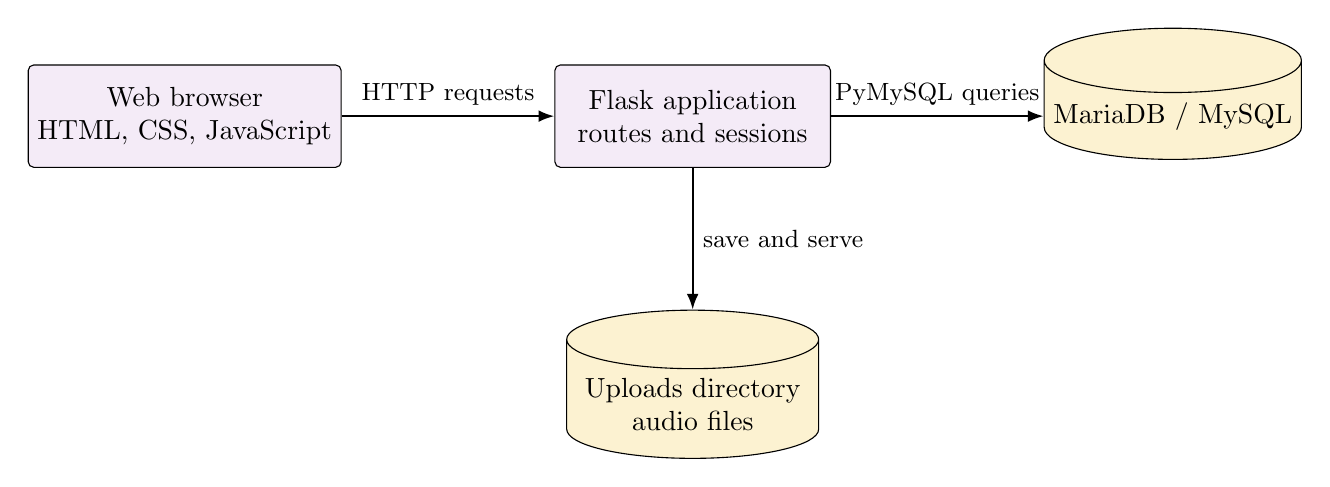
\begin{tikzpicture}[
  box/.style={draw, rounded corners=2pt, minimum width=35mm, minimum height=13mm, align=center, fill=brandpurple!8},
  store/.style={draw, cylinder, shape border rotate=90, aspect=0.25, minimum width=32mm, minimum height=16mm, align=center, fill=brandgold!18},
  arrow/.style={-{Latex[length=2mm]}, thick}
]
  \node[box] (browser) {Web browser\\HTML, CSS, JavaScript};
  \node[box, right=27mm of browser] (flask) {Flask application\\routes and sessions};
  \node[store, right=27mm of flask] (database) {MariaDB / MySQL};
  \node[store, below=18mm of flask] (uploads) {Uploads directory\\audio files};
  \draw[arrow] (browser) -- node[above, font=\small]{HTTP requests} (flask);
  \draw[arrow] (flask) -- node[above, font=\small]{PyMySQL queries} (database);
  \draw[arrow] (flask) -- node[right, font=\small]{save and serve} (uploads);
\end{tikzpicture}
\caption{High-level system architecture}
\end{figure}

\subsection{Database design}
The database contains users, songs, and ratings. Users can upload songs and submit ratings; each song belongs to one uploader. The unique pair \texttt{(song\_id, user\_id)} allows one editable rating per user and song. The \texttt{song\_ratings\_summary} view provides average ratings and counts.

\begin{figure}[H]
\centering
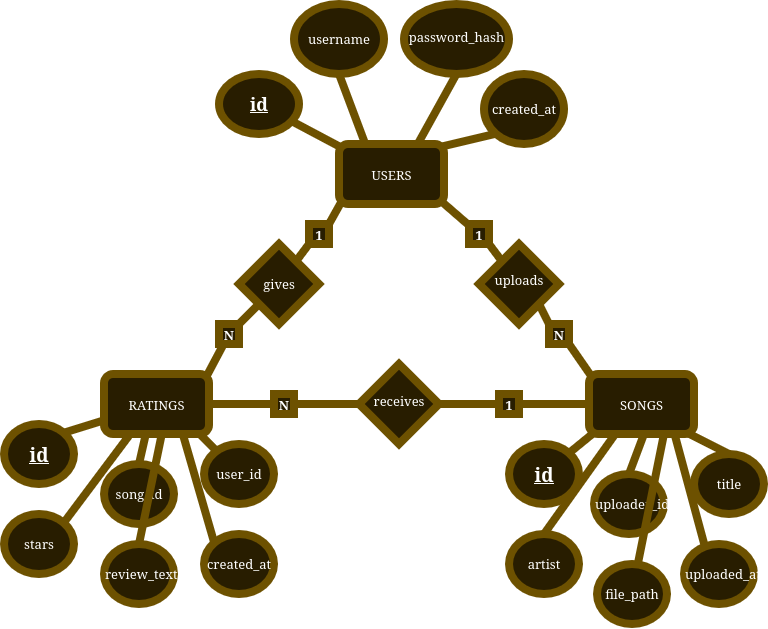
\includegraphics[width=\textwidth]{../docs/final.drawio.png}
\caption{Simplified entity-relationship model}
\end{figure}

\section{Implementation}

\subsection{Backend}
The Flask application in \texttt{app.py} retrieves songs, uploaders, and rating aggregates with SQL. Registration validates fields and stores a Werkzeug password hash. Login verifies the hash and stores the user identity in the session.

The upload route uses \texttt{login\_required}, \texttt{secure\_filename}, and a user/random filename prefix. Rating submissions validate the song and star range, then use an upsert so repeated submissions update the existing row.

\subsection{Frontend}
Jinja templates extend \texttt{base.html}. The library displays song metadata, an HTML audio player, and rating summaries. \texttt{app.js} coordinates audio playback and submits ratings asynchronously. CSS media queries support smaller screens.

\section{User Interface Evidence}
The following screenshots demonstrate the main user-facing workflows of
\projectname{}.

\subsection{User registration}
The registration page provides a focused form for creating an account with a
unique username and password. Existing members can use the login link below the
form.

\begin{figure}[H]
\centering
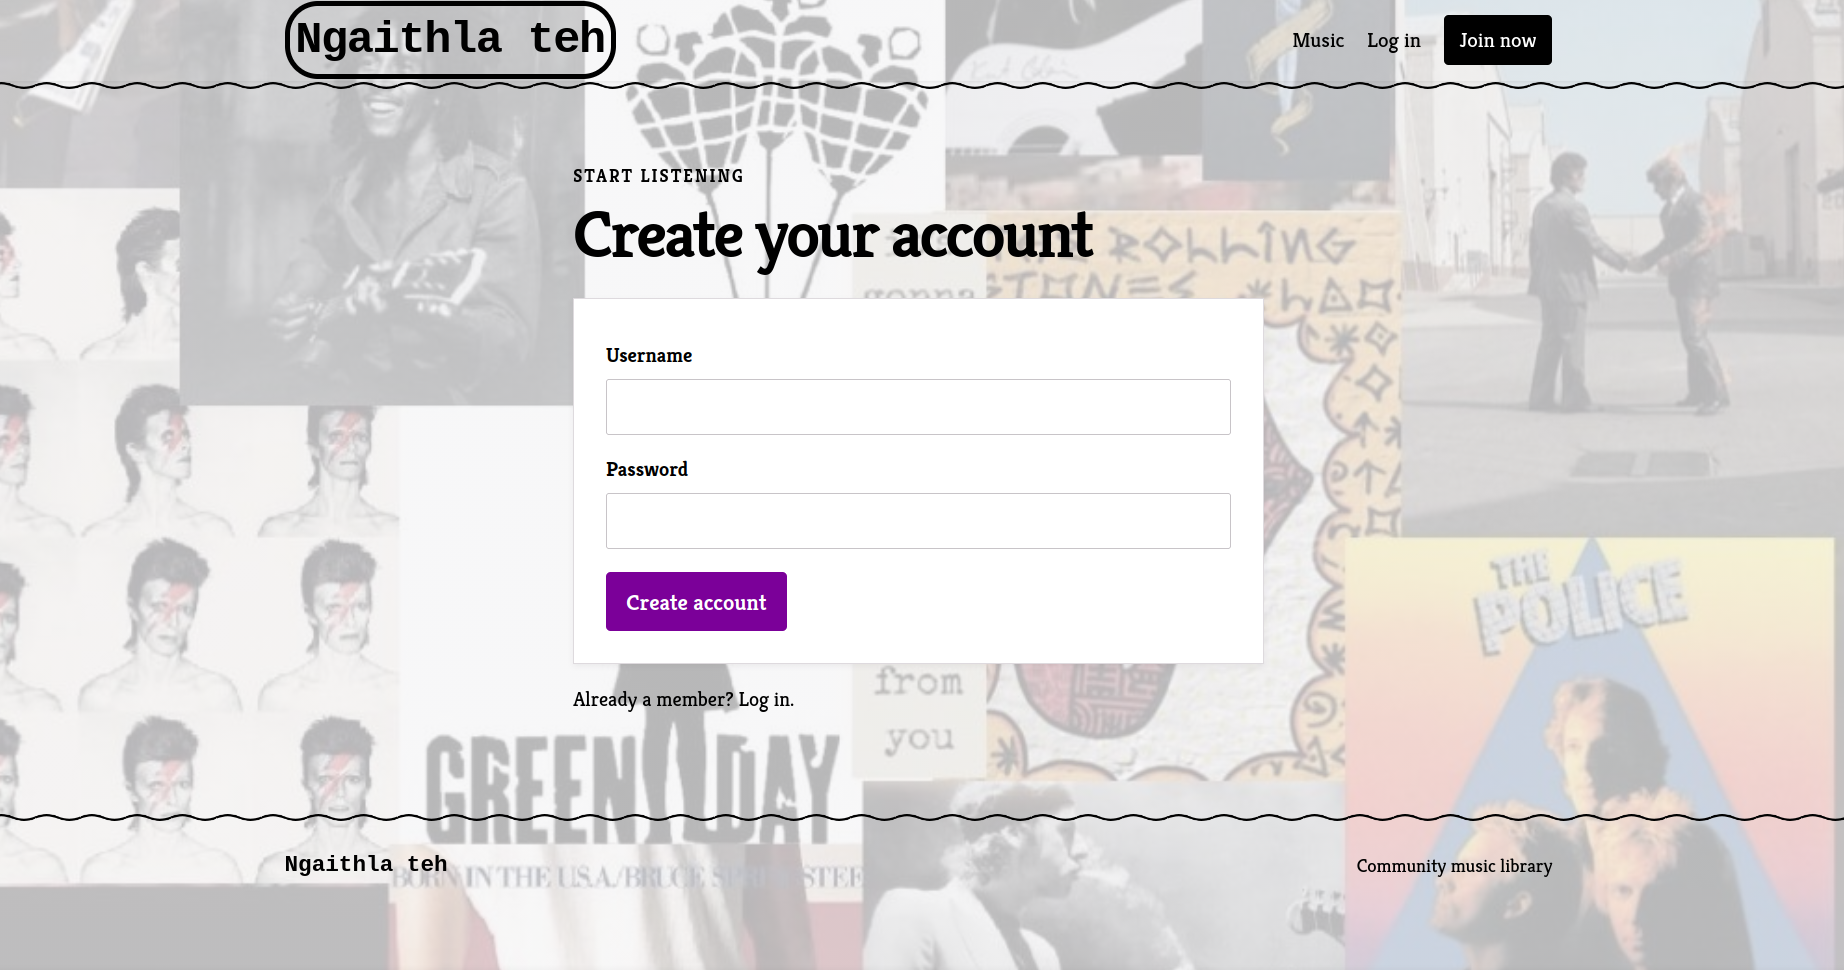
\includegraphics[width=\textwidth]{../docs/registration-page.png}
\caption{Registration page for creating a new user account}
\end{figure}

\subsection{Song upload}
Authenticated users can add a song by entering its title and artist name and
selecting an audio file. The upload form makes the contribution workflow
explicit before the file is stored in the application.

\begin{figure}[H]
\centering
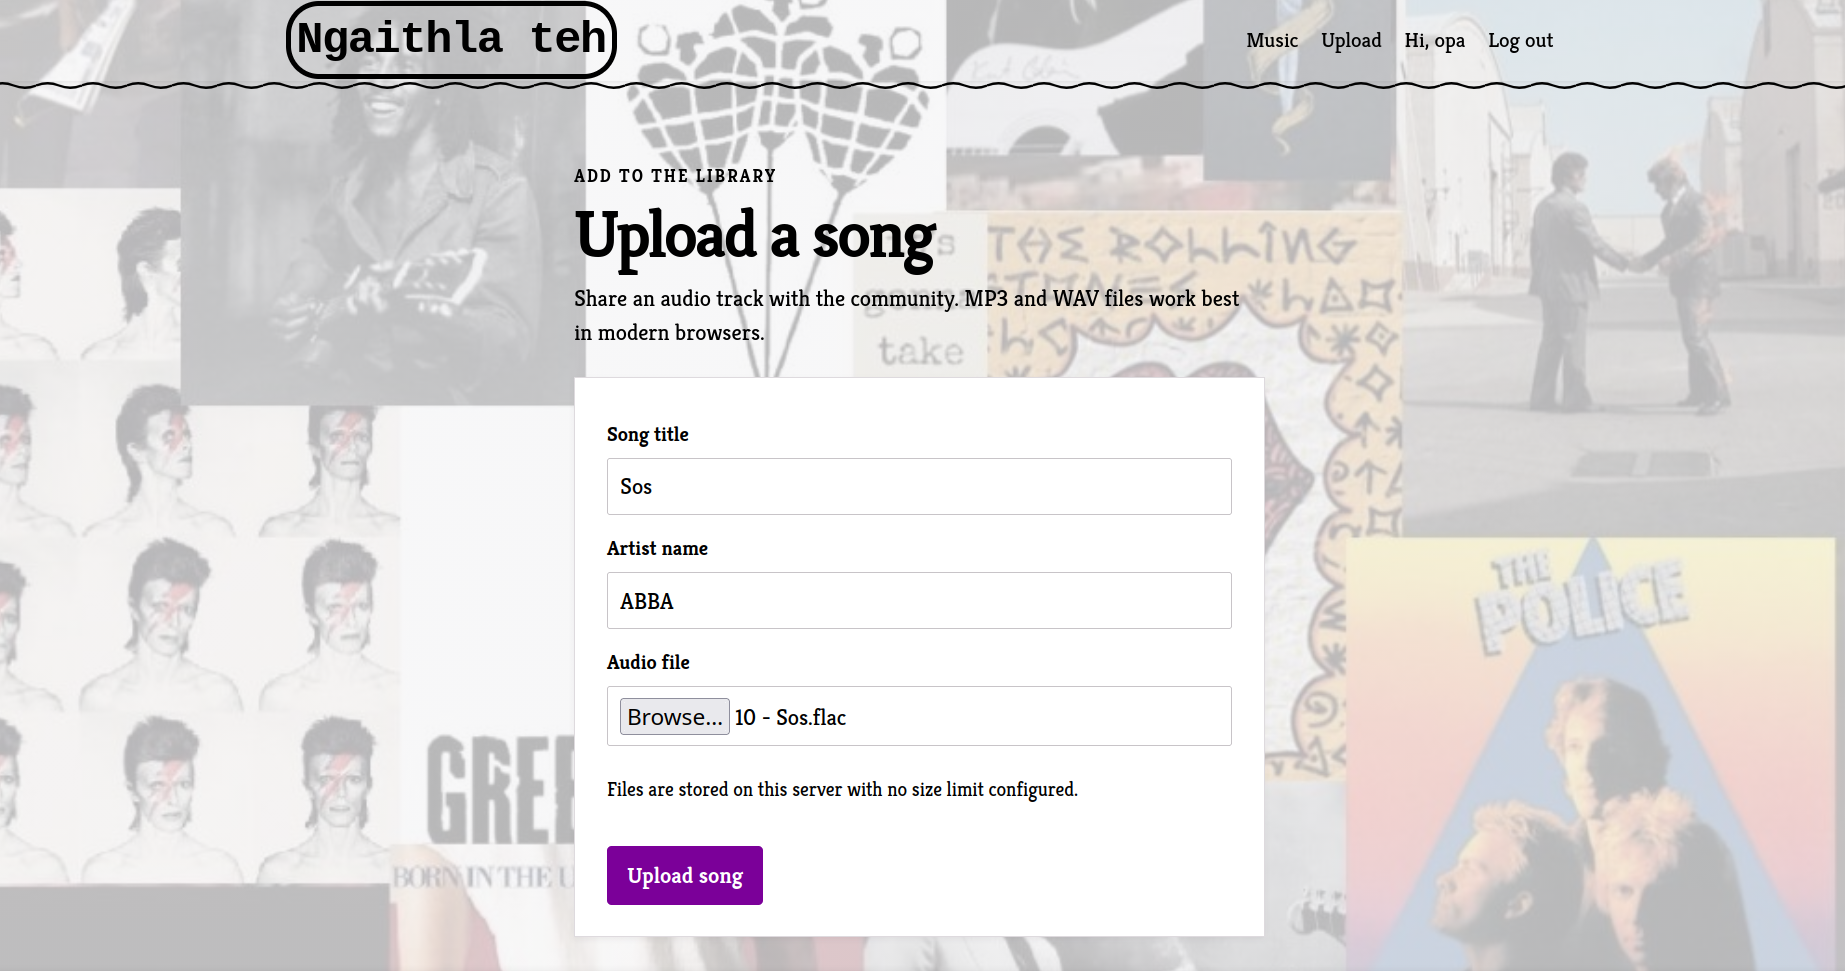
\includegraphics[width=\textwidth]{../docs/upload-form.png}
\caption{Upload form for adding a song to the community library}
\end{figure}

\subsection{Song rating and review}
The song view combines browser audio playback with the rating interface. A
listener can select a one-to-five-star rating, write an optional review, and
save the feedback for the selected song.

\begin{figure}[H]
\centering
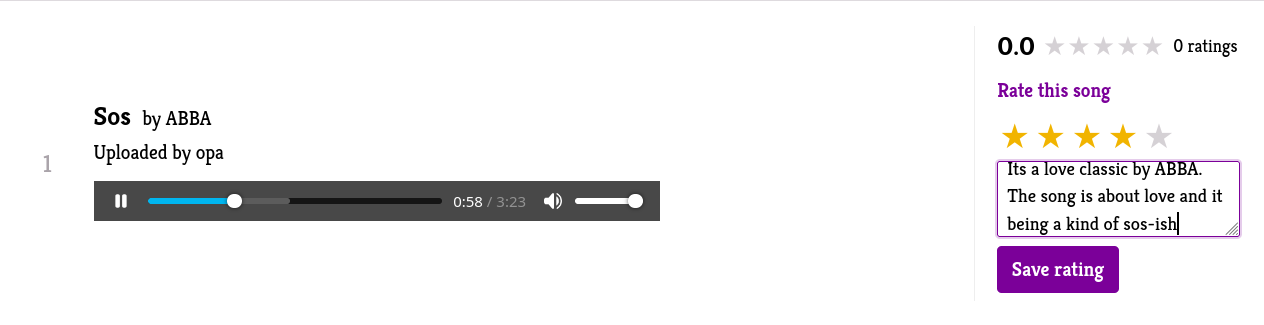
\includegraphics[width=\textwidth]{../docs/rating-song.png}
\caption{Song playback and rating interface}
\end{figure}

\subsection{Technology stack}
\begin{table}[H]
\centering
\begin{tabularx}{\textwidth}{lX}
\toprule
\textbf{Technology} & \textbf{Purpose} \\
\midrule
Python and Flask & Server-side routing, templates, sessions, and application logic \\
PyMySQL & Database connection and parameterized SQL execution \\
MariaDB / MySQL & Persistent relational data storage \\
HTML and Jinja & Page structure and server-rendered content \\
Vanilla JavaScript & Audio coordination and asynchronous rating submission \\
CSS & Responsive visual design and layout \\
Werkzeug & Password hashing and safe filename handling \\
\bottomrule
\end{tabularx}
\caption{Project technology stack}
\end{table}

\section{Testing and Evaluation}
The main workflows can be checked through a browser connected to the configured database.

\begin{table}[H]
\small
\centering
\begin{tabularx}{\textwidth}{p{0.25\textwidth}X p{0.14\textwidth}}
\toprule
\textbf{Test} & \textbf{Expected result} \\
\midrule
Registration and login & Valid users authenticate; duplicate or invalid credentials are rejected. \\
Upload and playback & An authenticated user can upload a track and play it in the browser. \\
Rating & A valid rating updates the summary and repeated submission does not duplicate it. \\
Invalid access and input & Protected routes redirect unauthenticated users and invalid stars are rejected. \\
\bottomrule
\end{tabularx}
\caption{Concise functional test matrix}
\end{table}

\section{Security and Data Integrity}
The implementation reduces common risks by using:
\begin{itemize}[leftmargin=*]
  \item Passwords are stored as hashes using Werkzeug rather than as plaintext.
  \item SQL values are passed as parameters to PyMySQL queries.
  \item Uploaded names are normalized with \texttt{secure\_filename}.
  \item Protected routes require a user ID in the session.
  \item Foreign keys cascade removal of dependent songs and ratings.
  \item The database constrains stars to the range one to five.
  \item The unique rating key prevents duplicate ratings for one user and song.
\end{itemize}

Before deployment, the development secret key must be replaced. Upload size and MIME type checks, CSRF protection, and moderation are also still required.

\section{Limitations and Future Work}
Future work includes:
\begin{enumerate}[leftmargin=*]
  \item server-side file validation and CSRF protection;
  \item search, sorting, pagination, and genre metadata;
  \item profiles, playlists, moderation, and administration; and
  \item automated tests and production object storage.
\end{enumerate}

\section{Conclusion}
\projectname{} is a focused community music library prototype. Flask, a relational schema, and a responsive browser interface provide the essential workflow for authentication, upload, playback, and feedback. Stronger validation, moderation, testing, and deployment controls are the main next steps.

\appendix
\section{Project Evidence Map}
\begin{table}[H]
\centering
\begin{tabularx}{\textwidth}{lX}
\toprule
\textbf{Report claim} & \textbf{Source in repository} \\
\midrule
Account creation and login & \texttt{app.py}, \texttt{templates/register.html}, \texttt{templates/login.html} \\
Song upload and playback & \texttt{app.py}, \texttt{templates/upload.html}, \texttt{templates/index.html} \\
Interactive ratings & \texttt{app.py}, \texttt{static/js/app.js} \\
Database entities and constraints & \texttt{schema.sql}, \texttt{docs/database-erd.drawio} \\
Installation and configuration & \texttt{README.md}, \texttt{requirements.txt} \\
\bottomrule
\end{tabularx}
\caption{Traceability from report content to project files}
\end{table}

\section{Selected Implementation Excerpt}
The following excerpt illustrates the database constraint that enforces one rating per user per song:

\begin{lstlisting}[language=SQL]
UNIQUE KEY unique_rating_per_user_per_song (song_id, user_id)
\end{lstlisting}

\end{document}